\chapter{Introduction}
% uncomment the following line to create an unnumbered chapter
%\chapter*{Introduction}\addcontentsline{toc}{chapter}{Introduction}\markboth{Introduction}{Introduction}
%---------------------------------------------------------------
\setcounter{page}{1}

A few sentences about progressive line of cryptocurrencies and attacks related to them. Tell about security audits and how it is time consuming. Then a bit about LLM, which is developed in parallel. THen tel labout desire to interesct these 2 fields and describe sections of this thesis. 

\chapter*{Objectives}

Tell a bit about what was done and list objectives that were fullfilled:

\begin{itemize}
    \item Common vulnerability patterns and existing auditing methodologies of Ethereum smart contracts were studied.
    \item A state of the art review on the integration of Large Language Models for automated reasoning and the development of AI-based auditing agents was conducted.
    \item A system that integrates an LLM into the security auditing workflow was designed with further implementation, testing and evaluation.
    \item The obtained results, limitations, and potential improvements of LLM-based auditing systems were discussed in the end.
\end{itemize}

\chapter{Ethereum}
This chapter introduces the foundations needed to understand Ethereum and the auditing methodologies developed in later chapters (TODO maybe change). It first explains generic \emph{blockchain} principles (as a technology family), then specializes to Ethereum’s execution model via the \emph{Ethereum Virtual Machine (EVM)} and the \emph{Solidity} language. The chapter closes with a concise taxonomy of common smart-contract vulnerabilities that will be referenced throughout the thesis.

\section{Overview}

Ethereum, formally launched in 2015, represents a significant evolution in blockchain technology. Originally proposed in a white paper by \textsc{Vitalik Buterin} in 2013/14, Ethereum extended the ledger-centric model into a full-fledged application layer offering smart contracts and decentralised applications (dApps) \cite{Buterin2013}. Rather than solely tracking value transfers, Ethereum enables arbitrary programmable logic through the EVM execution environment, while preserving the core blockchain properties of transparency, decentralisation and immutability \cite{wood2014yellow}. By doing so, it transformed the blockchain into a generalised state-transition machine, thereby broadening its applicability far beyond simple currency use-cases.

\subsection{Blockchain}

A blockchain is a distributed ledger maintained by a network of peer-to-peer nodes rather than a single central authority. It grows as a chain of blocks, each block holding a complete list of transaction records and containing a cryptographic link to its predecessor — when enough subsequent blocks accumulate, reversing or altering a transaction becomes infeasible. Participants use addresses instead of real-world identities, allowing transparency while preserving pseudonymity. Because every node holds a copy of the chain and the full history of transactions is publicly verifiable, the system enables auditability: flows of value can be traced, state transitions inspected and the integrity of past operations confirmed. In short, starting from the genesis block and continuing through every appended block, blockchain combines decentralization, tamper-resistance and verifiable history in one architecture \cite{blockchain}.


A blockchain offers immutability through cryptographic linking of blocks and the consensus mechanisms that govern their inclusion: once transactions are published and a block is finalised, reversing or deleting such entries becomes exceedingly difficult. Each block typically consists of two parts: a **header** and a **body**. The header contains metadata such as version, timestamp, the hash of the previous block, the Merkle-root of all transactions in the block, a nonce (or other proof field) and difficulty indicator. The body holds the transaction count and the individual transactions themselves \cite{blockchain_diagram_eth}.

\begin{figure}[!htbp]
    \centering
    \includegraphics[width=\linewidth]{images/blockchain_diagram_eth.pdf}
    \caption{Blockchain}
    \label{fig:blockchain_diagram_eth}
\end{figure}

 public blockchain, each n-ode could take part in the consensus process. And onlya selected set of nodes are responsible for validating theblock in consortium blockchain. As for private chain, it isfully controlled by one organization and the organizationcould determine the final consensus 

\subsection{Consensus mechanisms}

In a PoW system, network participants (miners) compete to solve computational puzzles (e.g., find a nonce so that the hash of the block header meets a target) and thereby propose the next valid block. :contentReference[oaicite:8]{index=8} In contrast, PoS selects block proposers (validators) based on their stake in the network (i.e., the amount of tokens locked up) rather than raw computing power, thereby altering the incentive, security and energy-profile of the system. :contentReference[oaicite:9]{index=9}

\subsubsection*{Proof of Work}
Proof-of-work (PoW) is an algorithm that sets the difficulty level and rules governing the activities of miners on PoW-based blockchains. Mining represents
the ’work’ needed to validate and append legitimate blocks to the blockchain.
This process is crucial as it directly affects the blockchain’s length, thereby
helping the network determine the most accurate progression of the chain.
As miners continue to solve complex mathematical problems, thereby adding
more blocks, the blockchain grows longer, which improves the network’s confidence in the current state of the ledger. This chain lengthening also increases
security by making altering any information in previous blocks increasingly
difficult. This consensus mechanism is used in the most popular blockchain
implementation, called Bitcoin.

\subsubsection*{Proof of Stake}
Proof of Stake (PoS) is an essential consensus algorithm that defines the rules
and mechanisms for participants in PoS-based blockchains. In PoS, the process of ’staking’—rather than mining—serves as the mechanism through which
validators are chosen to confirm transactions and create new blocks. Validators are selected based on the amount of cryptocurrency they hold and are
willing to ’stake’ as collateral. This process is critical as it helps ensure the
security and accuracy of the blockchain by encouraging validators to act honestly to avoid losing their stakes. As more blocks are validated and added to
the chain, the blockchain becomes longer and more robust, thereby upgrading
the network’s trust in the current ledger. This method increases the efficiency
of the validation process and reduces the energy consumption compared to
proof-of-work systems, making it a more environmentally friendly alternative.
The most used blockchain that uses the proof-of-stake mechanism is Ethereum

With a solid understanding of how blocks are structured and how consensus mechanisms (whether proof-of-work or proof-of-stake) enable nodes to agree upon the canonical chain, we now turn our attention to the next layer of the architecture: how transactions and smart contract code are actually executed

\section{Ethereum Virtual Machine}
The Ethereum Virtual Machine (EVM) is a deterministic state machine that executes the bytecode of the smart contract identically on all nodes \cite{wood2014yellow}. However, it is not Turing complete in the classical sense: execution is strictly resource-bounded by gas - every instruction has a metered gas cost, and execution halts once the supplied gas is exhausted. 
This gas-bounded execution guarantees termination and prevents non-halting or deliberately expensive programs from stalling the network; accordingly, the EVM is often described as \emph{quasi–Turing complete} (computationally universal only under a finite gas budget) \cite{antonopoulos2018mastering}\cite{wood2014yellow}.

\subsection{Gas}
Gas is the unit of account for computational effort in Ethereum. Each EVM opcode has an associated gas cost, and a transaction specifies an upper bound (gas limit) on how much gas may be consumed during its execution.

Gas serves three core purposes: 
\begin{itemize}
    \item \emph{metering} computation and storage, so that the use of the resources is paid for by the initiator of a transaction.
    \item \emph{DoS resistance} and spam prevention, because excessively resource-intensive executions become economically infeasible \cite{wood2014yellow}\cite{article_1559}.
    \item \emph{economic prioritization} of limited block space via fees
\end{itemize}

Since EIP-1559\footnote{\url{https://eips.ethereum.org/EIPS/eip-1559}}, each block includes a dynamically adjusted \emph{base fee} that is burned and a user-specified \emph{priority fee} (tip) paid to the block proposer. 
Users submit \texttt{maxFeePerGas} and \texttt{maxPriorityFeePerGas}; the effective price paid per gas equals \(\min(\texttt{maxFeePerGas}, \text{base fee} + \texttt{maxPriorityFeePerGas})\). 
Blocks have an elastic gas target and the base fee increases or decreases depending on recent block gas usage, stabilizing the fee market while preserving incentives.


\subsection{Architecture}

\begin{figure}[!htbp]
    \centering
    \includegraphics[width=\linewidth]{images/evm}
    \caption{Ethereum Virtual Machine illustration TODO REF.}
    \label{fig:evm}
\end{figure}

where 
\begin{itemize}
    \item Program Counter (PC) - component that tracks the current instruction that it is executing;
    \item EVM code - immutable compoennt holds the bytecode of the smart contract that is being executed.
    \item Account Storage - part of the persistent state of the blockchain where the data of smart contracts are stored permanently. There are two types of accounts in the Ethereum environment:\texttt{ (i) }Externally Owned Account (EOA) that is owned by any external entity. Most commonly, it is referred to as a user account; and\texttt{ (ii) }Smart Contract Account that is owned by a smart contract and often controlled by an EOA that interacts with the deployed smart contract \cite{Buterin2013}.
\end{itemize}

\subsection{Memory}

\begin{itemize}
    \item \textbf{Stack} - low-level memory structure that operates on a last-in, first-out (LIFO) principle. It stores small local variables and value types that are required for immediate execution. The stack is limited to 1024 elements, each 256 bits wide, and is accessible only through EVM opcodes or inline assembly. Careful management is essential, as exceeding its capacity causes the execution of the contract to fail \cite{evm_storage}.
    \item \textbf{Memory} - dynamic and expandable storage area allocated for each function execution, which is then discarded once the function has finished. Unlike the stack, which is restricted to temporary data storage, memory allows for more flexible and longer-lived data retention.
    \item \textbf{Storage} - persistent storage is associated with every smart contract and holds its state. Read and write operations in storage are relatively more expensive than those performed in memory. The data in storage are maintained as key-value pairs \cite{evm_storage_arxiv}.
    \item \textbf{Calldata} - read-only and immutable storage that holds function arguments and transaction data for the duration of a transaction call.
\end{itemize}

\section{Smart Contracts}

\subsection{Solidity}

\section{Ethereum Vulnerabilities Taxonomy}

\chapter{Foundations of LLMs for Code Analysis}

\chapter{State of the Art}
\section{Wake-AI}
\subsection{Wake framework}

\chapter{Proposed Methodology}

\chapter{Testing and Results}

\chapter{Conclusion}





% Do not forget to include Introduction
%---------------------------------------------------------------
\chapter{Introduction}
% uncomment the following line to create an unnumbered chapter
%\chapter*{Introduction}\addcontentsline{toc}{chapter}{Introduction}\markboth{Introduction}{Introduction}
%---------------------------------------------------------------

% The following environment can be used as a mini-introduction for a chapter. Use that any way it pleases you (or comment it out). It can contain, for instance, a summary of the chapter. Or, there can be a quotation.
\begin{chapterabstract}
	\lipsum[1]
\end{chapterabstract}

\lipsum[2][1-4]{} [1]

\lipsum[4]

%---------------------------------------------------------------
\section{Ut enim ad minim veniam}
%---------------------------------------------------------------

\lipsum[6-8]

\begin{figure}
\centering
%\includegraphics[scale=0.4]{pic/index}
\resizebox{\textwidth}{!}{
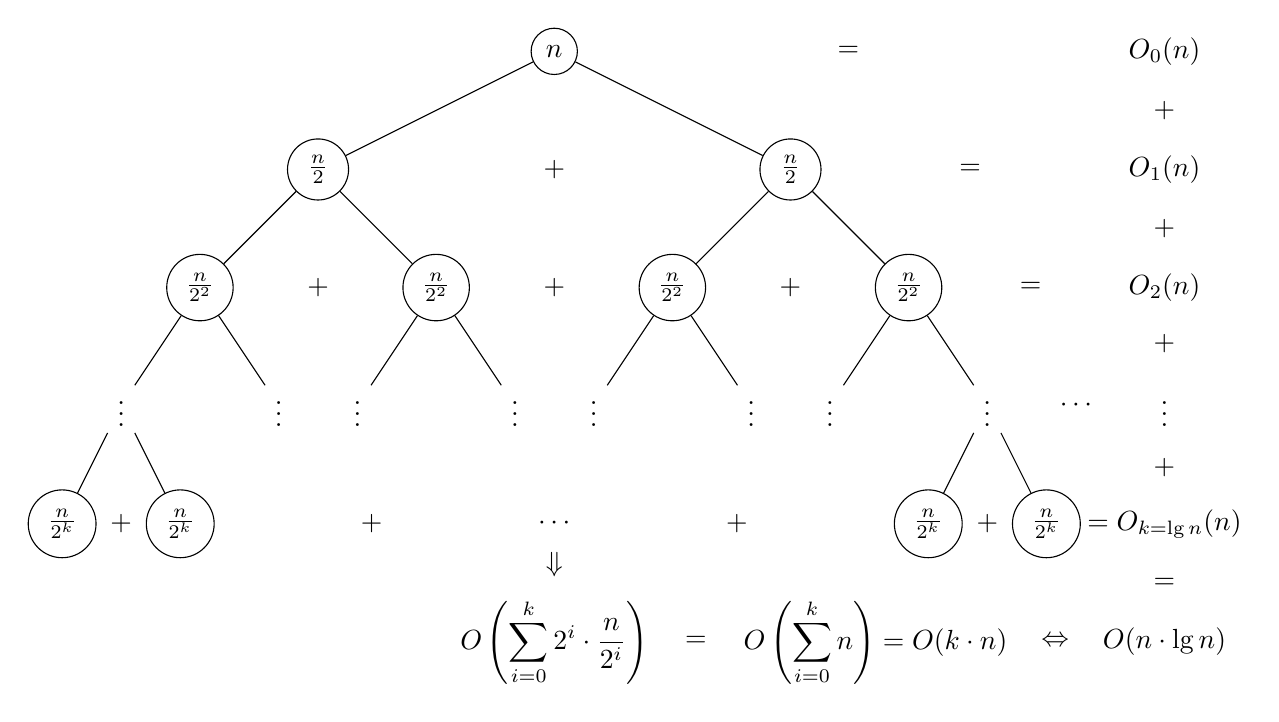
\begin{tikzpicture}[level/.style={sibling distance=60mm/#1}]
\node [circle,draw] (z){$n$}
  child {node [circle,draw] (a) {$\frac{n}{2}$}
    child {node [circle,draw] (b) {$\frac{n}{2^2}$}
      child {node {$\vdots$}
        child {node [circle,draw] (d) {$\frac{n}{2^k}$}}
        child {node [circle,draw] (e) {$\frac{n}{2^k}$}}
      } 
      child {node {$\vdots$}}
    }
    child {node [circle,draw] (g) {$\frac{n}{2^2}$}
      child {node {$\vdots$}}
      child {node {$\vdots$}}
    }
  }
  child {node [circle,draw] (j) {$\frac{n}{2}$}
    child {node [circle,draw] (k) {$\frac{n}{2^2}$}
      child {node {$\vdots$}}
      child {node {$\vdots$}}
    }
  child {node [circle,draw] (l) {$\frac{n}{2^2}$}
    child {node {$\vdots$}}
    child {node (c){$\vdots$}
      child {node [circle,draw] (o) {$\frac{n}{2^k}$}}
      child {node [circle,draw] (p) {$\frac{n}{2^k}$}
          child [grow=right] {node (q) {$ = O_{k = \lg n}(n)$} edge from parent[draw=none]
            child [grow=up] {node (r) {$\vdots$} edge from parent[draw=none]
              child [grow=up] {node (s) {$O_2(n)$} edge from parent[draw=none]
                child [grow=up] {node (t) {$O_1(n)$} edge from parent[draw=none]
                  child [grow=up] {node (u) {$O_0(n)$} edge from parent[draw=none]}
                }
              }
            }
            child [grow=down] {node (v) {$O(n \cdot \lg n)$}edge from parent[draw=none]}
        }
      }
    }
  }
};
\path (a) -- (j) node [midway] {+};
\path (b) -- (g) node [midway] {+};
\path (k) -- (l) node [midway] {+};
\path (k) -- (g) node [midway] {+};
\path (d) -- (e) node [midway] {+};
\path (o) -- (p) node [midway] {+};
\path (o) -- (e) node (x) [midway] {$\cdots$}
  child [grow=down] {
    node (y) {$O\left(\displaystyle\sum_{i = 0}^k 2^i \cdot \frac{n}{2^i}\right)$}
    edge from parent[draw=none]
  };
\path (q) -- (r) node [midway] {+};
\path (s) -- (r) node [midway] {+};
\path (s) -- (t) node [midway] {+};
\path (s) -- (l) node [midway] {=};
\path (t) -- (u) node [midway] {+};
\path (z) -- (u) node [midway] {=};
\path (j) -- (t) node [midway] {=};
\path (y) -- (x) node [midway] {$\Downarrow$};
\path (v) -- (y)
  node (w) [midway] {$O\left(\displaystyle\sum_{i = 0}^k n\right) = O(k \cdot n)$};
\path (q) -- (v) node [midway] {=};
\path (e) -- (x) node [midway] {+};
\path (o) -- (x) node [midway] {+};
\path (y) -- (w) node [midway] {$=$};
\path (v) -- (w) node [midway] {$\Leftrightarrow$};
\path (r) -- (c) node [midway] {$\cdots$};
\end{tikzpicture}}
\caption{Lorem ipsum dolor sit amet}\label{img:index}
\end{figure}

%---------------------------------------------------------------
\section{Ut enim ad minim veniam}
%---------------------------------------------------------------

\lipsum[2-4]

%---------------------------------------------------------------
\subsection{Ut enim ad minim veniam}
%---------------------------------------------------------------

Curabitur ligula sapien, pulvinar a vestibulum quis, facilisis vel sapien. Duis condimentum augue id magna semper rutrum. Aliquam ornare wisi eu metus. Fusce aliquam vestibulum ipsum. Vivamus ac leo pretium faucibus~\ref{img:index}.

\begin{itemize}
    \item Ut enim ad minim veniam, quis nostrud
    \item Ut enim ad minim 
    \item Ut enim ad minim veniam, quis 
    \begin{itemize}
        \item Ut enim ad
        \item Ut enim ad
        \begin{itemize}
            \item Ut enim 
            \item Ut enim 
            \begin{itemize}
            \item Ut enim 
            \item Ut enim 
        \end{itemize}
        \end{itemize}
    \end{itemize}
\end{itemize}

\section{Class aptent taciti}


Even though dark mode can be very nice for websites and apps, it does not look good when printed. Consider using white mode when print-screening dark-moded content. The contrast with the white page is too big, as seen in Figure~\ref{fig:Darkmode}.

\begin{figure}[!htbp]
    \centering
    \includegraphics[width=\linewidth]{images/darkmode}
    \caption{White and dark mode comparison.~\cite{darkMode}}
    \label{fig:Darkmode}
\end{figure}


\subsection{Class aptent taciti}

\lipsum[6-7]

\begin{enumerate}
    \item Ut enim ad minim veniam, quis nostrud
    \item Ut enim ad minim 
    \item Ut enim ad minim veniam, quis 
    \begin{enumerate}
        \item Ut enim ad
        \item Ut enim ad
        \begin{enumerate}
            \item Ut enim 
            \item Ut enim 
            \begin{enumerate}
            \item Ut enim 
            \item Ut enim 
        \end{enumerate}
        \end{enumerate}
    \end{enumerate}
\end{enumerate}


%---------------------------------------------------------------
\section{Ut enim ad minim veniam, quis nostrud}
%---------------------------------------------------------------

Ut enim ad minim veniam, quis nostrud exercitation ullamco laboris nisi ut aliquip ex ea commodo consequat. Nulla non arcu lacinia neque faucibus fringilla. Vestibulum erat nulla, ullamcorper nec, rutrum non, nonummy ac, erat. Aliquam erat volutpat. Proin pede metus, vulputate nec, fermentum fringilla, vehicula vitae, justo.\footnote{Ut enim ad minim veniam, quis nostrud exercitation.} Etiam dictum tincidunt diam. In laoreet, magna id viverra tincidunt, sem odio bibendum justo, vel imperdiet sapien wisi sed libero. Nulla est. Maecenas fermentum, sem in pharetra pellentesque, velit turpis volutpat ante, in pharetra metus odio a lectus. Duis aute irure dolor in reprehenderit in voluptate velit esse cillum dolore eu fugiat nulla pariatur. 

\begin{lstlisting}[caption={Zbytečný kód},label=list:8-6,captionpos=b,float,abovecaptionskip=-\medskipamount,abovecaptionskip=\medskipamount,language=C]
    #include<stdio.h>
    #include<iostream>
    // A comment
    int main(void)
    {
        printf("Hello World\n");
        return 0;
    }
\end{lstlisting}

%%%%%%%%%%%%%%%%%%%%%%%%%%%%%%%%%
% alternative using package minted for source highlighting
% package minted requires execution with `-shell-escape'
% e.g., `xelatex -shell-escape ctufit-thesis.tex'
% \begin{listing}
% \begin{minted}{C}
%     #include<stdio.h>
%     #include<iostream>
%     // A comment
%     int main(void)
%     {
%         printf("Hello World\n");
%         return 0;
%     }
% \end{minted}
% \caption{Zbytečný kód}\label{list:8-6}
% \end{listing}
% %%%%%%%%%%%%%%%%%%%%%%%%%%%%%%%%%
Nullam feugiat, turpis at pulvinar vulputate, erat libero tristique tellus, nec bibendum odio risus sit amet ante. Aenean id metus id velit ullamcorper pulvinar. Fusce wisi. Integer lacinia. Aliquam id dolor. Pellentesque pretium lectus id turpis. Suspendisse sagittis ultrices augue. In laoreet, magna id viverra tincidunt, sem odio bibendum justo, vel imperdiet sapien wisi sed libero. Sed ac dolor sit amet purus malesuada congue.~\cite{Crochemore2002}

Class aptent taciti sociosqu ad litora torquent per conubia nostra, per inceptos hymenaeos. Fusce suscipit libero eget elit. Etiam dui sem, fermentum vitae, sagittis id, malesuada in, quam. Aliquam id dolor. Curabitur bibendum justo non orci. Duis viverra diam non justo. Curabitur ligula sapien, pulvinar a vestibulum quis, facilisis vel sapien. Duis condimentum augue id magna semper rutrum. Aliquam ornare wisi eu metus. Fusce aliquam vestibulum ipsum. Vivamus ac leo pretium faucibus.~\cite{Motwani2014}

%---------------------------------------------------------------
\subsection{Ut enim ad minim veniam, quis nostrud}
%---------------------------------------------------------------

Ut enim ad minim veniam, quis nostrud exercitation ullamco laboris nisi ut aliquip ex ea commodo consequat. Nulla non arcu lacinia neque faucibus fringilla. Vestibulum erat nulla, ullamcorper nec, rutrum non, nonummy ac, erat. Aliquam erat volutpat. Proin pede metus, vulputate nec, fermentum fringilla, vehicula vitae, justo. Etiam dictum tincidunt diam. In laoreet, magna id viverra tincidunt, sem odio bibendum justo.~\cite{Sestakova2018} 

\begin{table}\centering
\begin{tabular}{l|l|c|c}
	Typ		& Prostředí		& \LaTeX{}ovská zkratka	& \TeX{}ovská zkratka	\tabularnewline \hline 
 	Text		& \verb|math|		& \verb|\(...\)|	& \verb|$...$|	\tabularnewline \hline
 	Displayed	& \verb|displaymath|	& \verb|\[...\]|	& \verb|$$...$$|	\tabularnewline 
\end{tabular}
\caption[Příklad tabulky]{Zadávání matematiky}
\label{tab:matematika}
\end{table}


Nulla est. Maecenas fermentum, sem in pharetra pellentesque, velit turpis volutpat ante, in pharetra metus odio a lectus. Duis aute irure dolor in reprehenderit in voluptate velit esse cillum dolore eu fugiat nulla pariatur. Nullam feugiat, turpis at pulvinar vulputate, erat libero tristique tellus, nec bibendum odio risus sit amet ante. Aenean id metus id velit ullamcorper pulvinar. 

\subsubsection{Class aptent taciti}

\begin{definition}[Optional label]
Class aptent taciti sociosqu ad litora torquent per conubia nostra, per inceptos hymenaeos. Fusce suscipit libero eget elit. Etiam dui sem, fermentum vitae, sagittis id, malesuada in, quam. Aliquam id dolor. Curabitur bibendum justo non orci.
\end{definition}

\begin{example}
Class aptent taciti sociosqu ad litora torquent per conubia nostra, per inceptos hymenaeos. Fusce suscipit libero eget elit. Etiam dui sem, fermentum vitae, sagittis id, malesuada in, quam. Aliquam id dolor. Curabitur bibendum justo non orci.
\end{example}

\paragraph{Nadpis 5. úrovně}

\begin{theorem}
Class aptent taciti sociosqu ad litora torquent per conubia nostra, per inceptos hymenaeos. Fusce suscipit libero eget elit. Etiam dui sem, fermentum vitae, sagittis id, malesuada in, quam. Aliquam id dolor. Curabitur bibendum justo non orci.
\end{theorem}

\begin{proof}
Fusce suscipit libero eget elit. Etiam dui sem, fermentum vitae, sagittis id, malesuada in, quam. Aliquam id dolor. Curabitur bibendum justo non orci.
\end{proof}

\paragraph{Level 5 heading}

\begin{corollary}
Fusce suscipit libero eget elit. Etiam dui sem, fermentum vitae, sagittis id, malesuada in, quam. Aliquam id dolor. Curabitur bibendum justo non orci.
\end{corollary}

\begin{proposition}
Fusce suscipit libero eget elit. Etiam dui sem, fermentum vitae, sagittis id, malesuada in, quam. Aliquam id dolor. Curabitur bibendum justo non orci.
\end{proposition}

\begin{note}
Fusce suscipit libero eget elit. Etiam dui sem, fermentum vitae, sagittis id, malesuada in, quam. Aliquam id dolor. Curabitur bibendum justo non orci.
\end{note}

\begin{remark}
Fusce suscipit libero eget elit. Etiam dui sem, fermentum vitae, sagittis id, malesuada in, quam. Aliquam id dolor. Curabitur bibendum justo non orci.
\end{remark}

\begin{lemma}
Class aptent taciti sociosqu ad litora torquent per conubia nostra, per inceptos hymenaeos. Fusce suscipit libero eget elit. Etiam dui sem, fermentum vitae, sagittis id, malesuada in, quam. Aliquam id dolor. Curabitur bibendum justo non orci.
\end{lemma}

\lipsum[1-2]

% \subsection{Class aptent taciti sociosqu}
% 
% \lipsum[4-5]

%---------------------------------------------------------------
\chapter{Lorem ipsum}
%---------------------------------------------------------------

\begin{chapterabstract}
	Lorem ipsum dolor sit amet, consectetuer adipiscing elit. Curabitur sagittis hendrerit ante. Class aptent taciti sociosqu ad litora torquent per conubia nostra, per inceptos hymenaeos. Cras pede libero, dapibus nec, pretium sit amet, tempor quis. Sed vel lectus. Donec odio tempus molestie, porttitor ut, iaculis quis, sem. Cras pede libero, dapibus nec, pretium sit amet, tempor quis. Sed vel lectus. 
\end{chapterabstract}

Lorem ipsum dolor sit amet, consectetuer adipiscing elit. Curabitur sagittis hendrerit ante. Class aptent taciti sociosqu ad litora torquent per conubia nostra, per inceptos hymenaeos. Cras pede libero, dapibus nec, pretium sit amet, tempor quis. Sed vel lectus. Donec odio tempus molestie, porttitor ut, iaculis quis, sem. Suspendisse sagittis ultrices augue. Donec ipsum massa, ullamcorper in, auctor et, scelerisque sed, est. In sem justo, commodo ut, suscipit at, pharetra vitae, orci. Pellentesque pretium lectus id turpis.~\cite{Kopka2004}

\section{Donec odio tempus molestie}

\lipsum[2]~\cite{def:1, def:2}

\subsection{Class aptent taciti}

\lipsum[2-3]

\begin{description}
\item[Kapitola 1] Lorem ipsum dolor sit amet, consectetuer adipiscing elit. Curabitur sagittis hendrerit ante. Class aptent taciti sociosqu ad litora tor\-quent per conubia nostra, per inceptos hymenaeos. Cras pede libero, dapibus nec, pretium sit amet, tempor quis.

\item[Kapitola 2] Lorem ipsum dolor sit amet, consectetuer adipiscing elit. Curabitur sagittis hendrerit ante. Class aptent taciti sociosqu ad litora tor\-quent per conubia nostra, per inceptos hymenaeos. Cras pede libero, dapibus nec, pretium sit amet, tempor quis.

\item[Kapitola 3] Lorem ipsum dolor sit amet, consectetuer adipiscing elit. Curabitur sagittis hendrerit ante. Class aptent taciti sociosqu ad litora tor\-quent per conubia nostra, per inceptos hymenaeos. Cras pede libero, dapibus nec, pretium sit amet, tempor quis.

\item[Kapitola 4] Lorem ipsum dolor sit amet, consectetuer adipiscing elit. Curabitur sagittis hendrerit ante. Class aptent taciti sociosqu ad litora tor\-quent per conubia nostra, per inceptos hymenaeos. Cras pede libero, dapibus nec, pretium sit amet, tempor quis.~\cite{jakZiskatAcko}
\end{description}

\lipsum[2]

\section{Lorem ipsum dolor sit amet}

\lipsum[3-5]
